\chapter{Dispersão de Ondas Rayleigh}

\section{Introdução}

Os métodos para determinar a estrutura sísmica da Terra, em particular os métodos tomográficos, baseiam-se num princípio simples: a determinação das velocidades de propagação das ondas sísmicas e a procura de um modelo que melhor se ajuste às velocidades encontradas. A resolução dos modelos obtidos depende do tipo de onda utilizado e da geometria espacial das estações sismigráficas segundo à fonte do sinal. \cite{aki_space_1957} propôs a utilização do ruído sísmico ambiental para medir a dispersão das ondas Rayleigh e Love nas camadas mais superficiais. Somente \cite{campillo_long-range_2003}  e \cite{shapiro_emergence_2004} mostraram, pela primeira vez, a  presença de ondas superficiais nas correlações cruzadas entre pares de estações.

\cite{campillo_long-range_2003}, \cite{shapiro_emergence_2004} e, principalmente, \cite{wapenaar_retrieving_2004} mostram que pode-se recuperar a resposta elástica da Terra a partir da correlação cruzada entre dois pontos em  um campo de ondas difuso ou aleatório. Essa resposta é aproximada como a Função de Green, como é mostrada na equação \ref{crosscorrelation}. 

\cite{boschi_measuring_2013} define a correlação cruzada ($C_{xy}(t,\omega)$) como: 
\begin{eqnarray}
\label{crosscorrelation}
C_{xy}(t,\omega) = \frac{1}{2\pi}\int_{-T}^{T}u(x,t,\omega)u(y,t+\tau,\omega) d\tau
\end{eqnarray}

onde $u$ são sinais registrados em duas estações nas posições $x$ e $y$, $t$ é o tempo, $\omega$ é a frequência, $\tau$ é o atraso e o parâmetro T define o tamanho da janela que a correlação cruzada será computada.
\\

Por possuir inúmeras vantagens em relação aos métodos de análise tradicionais, o número de artigos analisando a dispersão de ondas de superfície cresceu bastante. \cite{shapiro_emergence_2004} lista as seguintes vantagens: as medidas podem ser realizadas em qualquer direção de propagação e não estão limitadas à geometria fonte-receptor; não dependem da localização da fonte; a zona de sensibilidade destas medições situa-se na região que fica entre as duas estações; pode-se analisar pequenos períodos se existirem estações relativamente próximas umas das outras.

\cite{shapiro_emergence_2004} testaram se as funções de Green podem ser extraídas do ruído sísmico ambiental. Neste teste eles selecionaram um
período relativamente calmo no nível de atividade sísmica mundial, onde não ocorreram sismos com magnitude menor que 7. Com esses registos contínuos da componente vertical das estações ANMO e CCM, vistas na Figura \ref{shapiro}-a). Com isso calcularam a correlação cruzada para diferentes bandas de período, mostrado na Figura \ref{shapiro}-b), e aplicaram a análise tempo/frequência para calcular a velocidade de grupo das ondas de superfície segundo \cite{levshin_automated_2001}. \cite{shapiro_emergence_2004}  compararam as características de dispersão do sinal emergente com mapas preditos para o mesmo trajeto.  Nesta comparação, verificaram que os resultados obtidos para os dois casos são semelhantes.

\begin{figure}[!ht]
\centering
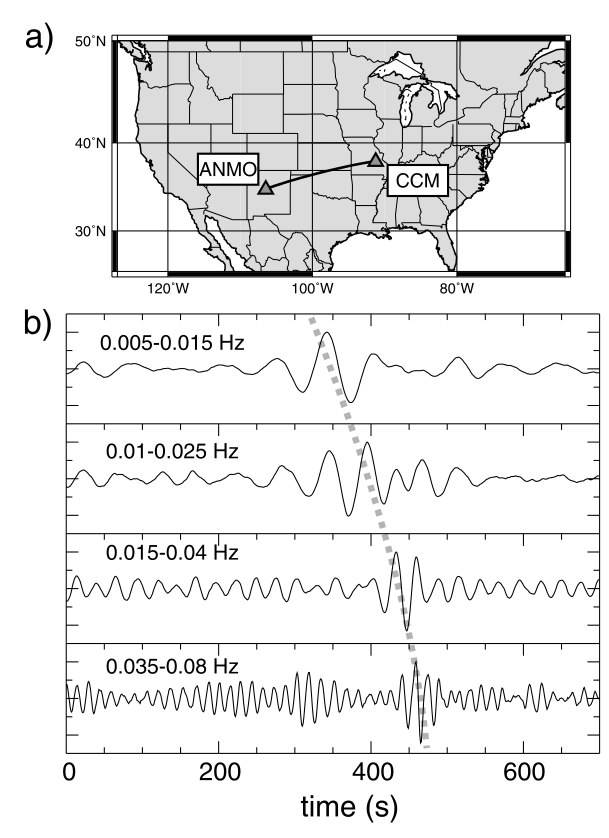
\includegraphics[scale=0.7]{Figs/shapiro2004.png}
\caption{a) Mapa mostrando a localização das estações. b) Correlações cruzadas da componente vertical dos registros com diferentes filtros de passa-banda, indicados na parte esquerda superior. Linha pontilhada dá ênfase na dispersão do sinal emergente. Extraído de \cite{shapiro_emergence_2004}.}
\label{shapiro}
\end{figure} 

\section{Processamento}

Para o processamento dos dados utilizou-se o código escrito pelo Professor Bruno Goutorbe. Tal código engloba a preparação dos dados, o cálculo da correlação, a análise Tempo/frequência e também a inversão tomográfica.  O código está disponível no GitHub no seguinte repositório: https://github.com/bgoutorbe/seismic-noise-tomography.

Todo o fluxo de preparação e processamento dos dados  baseia-se no trabalho de \cite{bensen_processing_2007}. Porém há alterações na filtragem espectral utilizada neste trabalho, devido a utilização de média a alta frequência no processamento.

\begin{figure}[!ht]
\centering
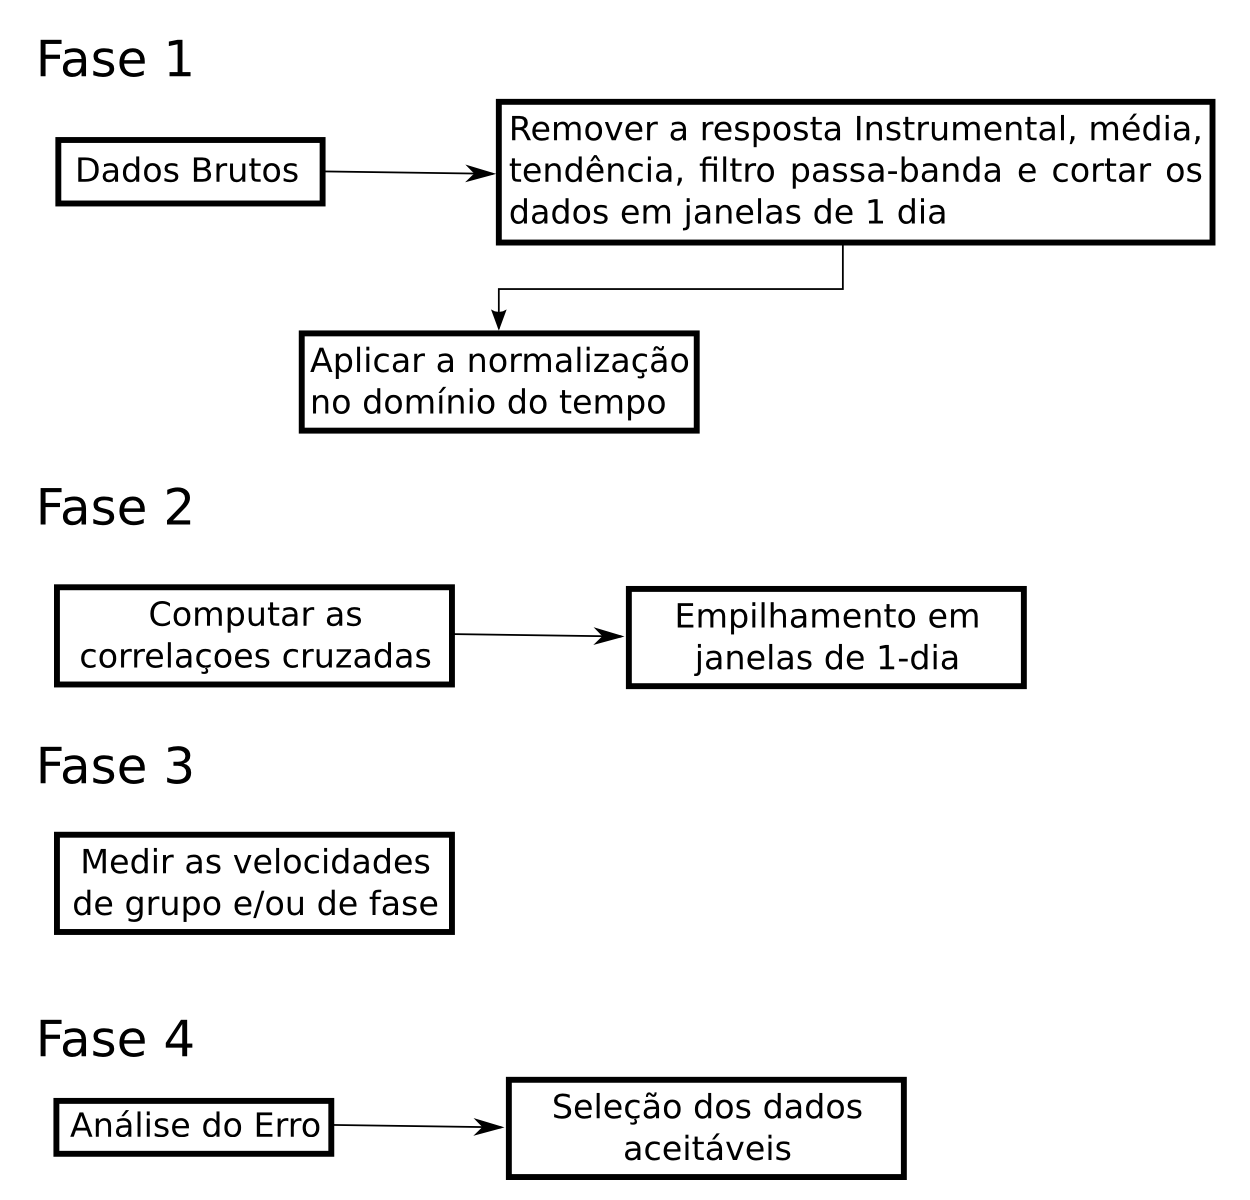
\includegraphics[scale=0.8]{Figs/fluxograma_bensen2007.png}
\caption[Representação esquemática do processamento.]{Representação esquemática do processamento. Fase 1 - etapas que involvem a preparação dos dados antes da correlação. Fase 2 - esboços do processo de correlação cruzadae empilhamento. Fase 3 -Medidas de dispersão. Fase 4 - Análise do Erro e seleção de dados aceitáveis. Adaptado de \cite{bensen_processing_2007}.}
\label{fluxograma_bensen2007}
\end{figure} 

\subsection{Preparação dos dados para cada estações}

\cite{bensen_processing_2007} cita que a primeira fase do processamento  é feita para preparar os dados da forma da onda de cada estação individualmente, faz-se isso para acentuar o ruído ambiental de banda larga tentando remover os sinais de terremoto e de irregularidades instrumental que tendem a ocultar o ruído ambiental.

Segundo \cite{bensen_processing_2007}, séries temporáis diárias com menos que 80\% do registro devem ser rejeitadas, mas isso varia de acordo com a discretização do usuário. No caso desse trabalho foram utilizados séries  temporáis diárias com 99\% do registro com o propósito de usar a interpolação o míńimo possível.

Um passo importante na preparação dos dados é a "normalização temporal" ou "normalização no domínio do tempo", \cite{bensen_processing_2007}. Isto é feito para reduzir na correlação cruzada os efeitos de terremotos, irregularidades instrumentais e fontes de ruído não-estacionários próximos á estação. \cite{bensen_processing_2007} compara cinco métodos diferentes para a normalização temporal, como observado na Figura \ref{temporal_norma}.

\begin{figure}[!ht]
\centering
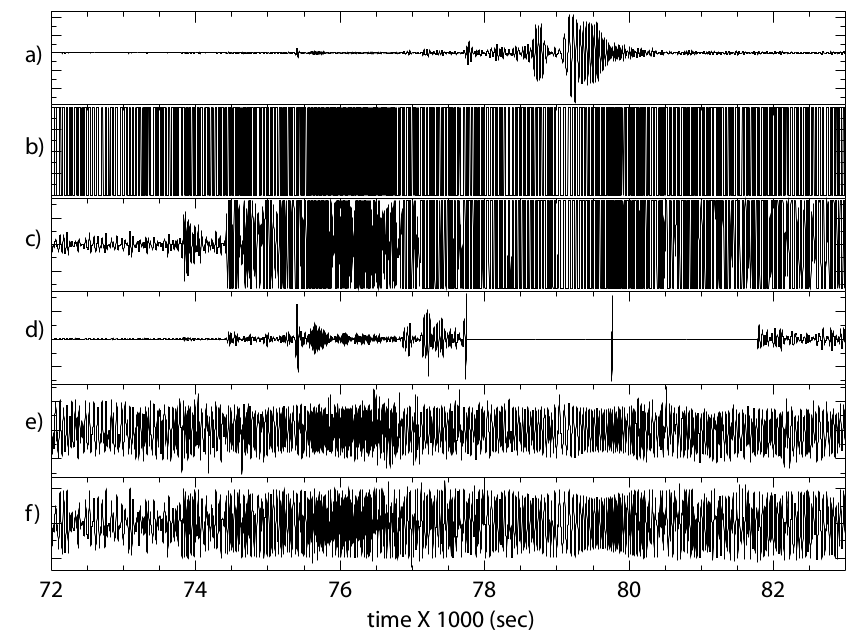
\includegraphics[scale=0.55]{Figs/temporal_norma.png}
\caption[Formas de onda mostrando exemplos de cinco tipos de normalização no dominio do tempo.]{Formas de onda mostrando exemplos de cinco tipos de normalização no dominio do tempo testadas por \cite{bensen_processing_2007}. Os exemplos estão com o filtro passa-banda entre 20 e 100 segundos e mostram a contaminação por sinais de terremoto. (a)  Dado bruto mostrando 3 horas de dados janelados em torno de um grande terremoto (M = 7.2, Afeganistão) registrado na estação ANMO. (b) Normalização 1-bit.(c) Forma de onda cortada, onde o limiar de recorte é igual ao rms da amplitude do sinal de um dado dia. (d) Evento detectado e removido automaticamente. (e) Normalização da média absoluta móvel. (f) Normalização ‘\textit{Water level}’ . Retirado de \cite{bensen_processing_2007}.}
\label{temporal_norma}
\end{figure} 

Terremotos geram grandes impecílios na automatização do processamento, pois eles ocorrem irregularmente e apenas grandes terremotos são encontrados nos catálogos globais, como visto na na Figura \ref{temporal_norma}-a. Então a remoção dos sinais dos terremotos tem que ser adaptativa aos dados. Muitos estudos aplicam a técnica da "normalização 1-bit", como observado na Figura \ref{temporal_norma}-b, em que somente o sinal da série temporal é retido (+1 ou -1) e a amplitude é completamente ignorada. Neste trabalho foi aplicado a "normalização da média absoluta móvel", esta produz uma razão sinal-ruído maior que a normalização 1-bit no conjunto de dados utilizados, estando de acordo com estudos de \cite{seats_improved_2012}.

\subsection{Normalização espectral ou braqueamento}

O ruído sísmico ambiente não é branco no domínio da frequência, ou seja, tem frequências que se destacam. \cite{bensen_processing_2007} cita que a normalização espectral atua para alargar a banda do sinal de ruído ambiental nas correlações cruzadas e também combate a degradação causada por fontes persistentes.

A janela temporal que \cite{bensen_processing_2007} utiliza em seu trabalho é de 7 a 150 segundos, porém quando a distância entre as estações é pequena ($\simeq 20 km$) é necessário utilizar períodos mais curtos, como é o caso desse trabalho. A janela temporal utilizada é de 2 a 50 segundos, logo há inclusão de ruído de alta frequência.

Com a necessidade de preservar este ruído de alta frequência não foi aplicada a normalização espectral.


\subsection{Correlação Cruzada, Empilhamento e  Sinal emergente}

Após preparar as séries temporais diárias a próxima fase, como visto na Figura \ref{fluxograma_bensen2007}, é computar as correlações cruzadas e o empilhamento. \cite{bensen_processing_2007} mostra que mesmo as distâncias das estações sendo muito longas ou curtas deve-se fazer a correlação entre todas as estações possíveis e no futuro fazer a seleçã o das medidas aceitáveis. O número total de pares de estações possíveis é dado por $n(n-1)/2$, onde $n$ é o número de estações.

\begin{figure}[!ht]
\centering
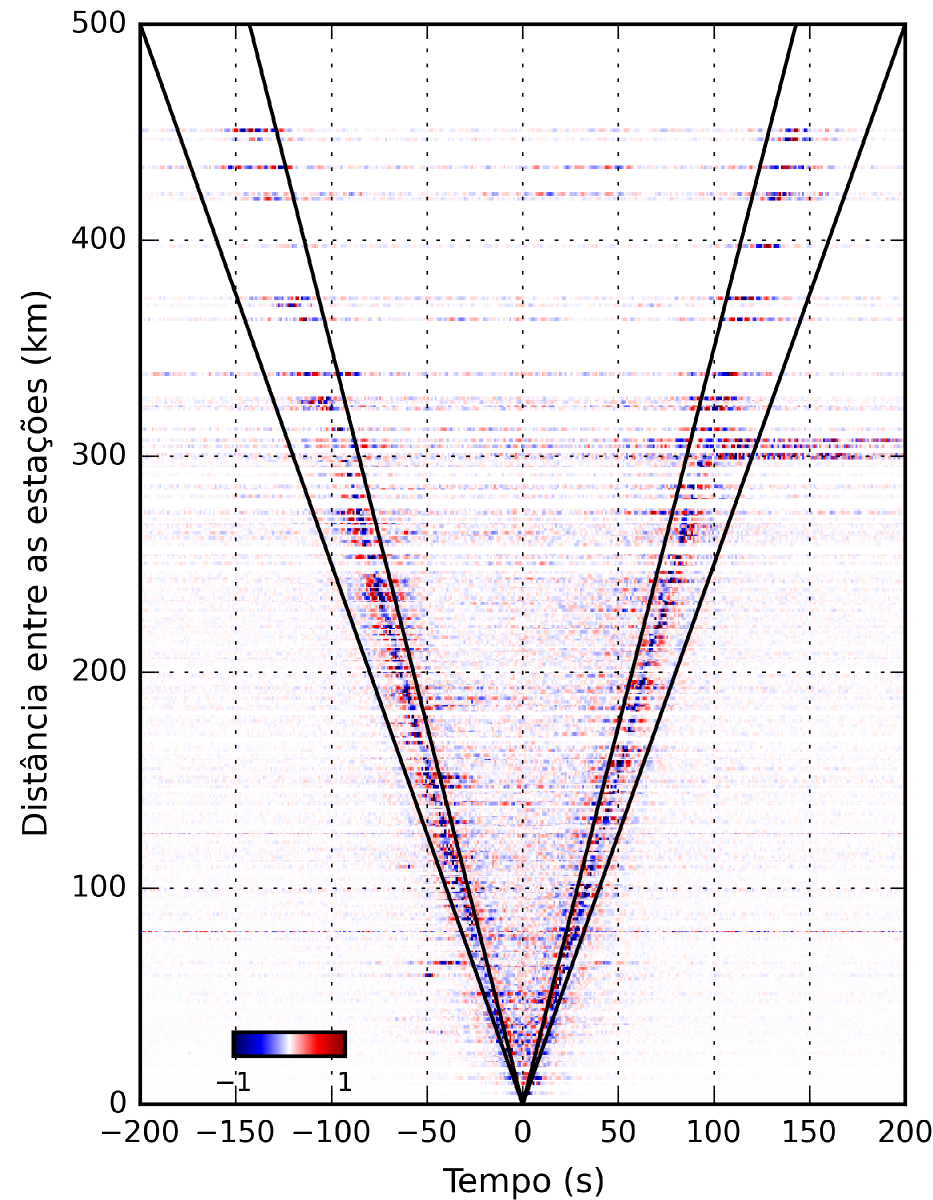
\includegraphics[scale=0.11]{Figs/correlaca_cruzada.png}
\caption[Correlações cruzadas de acordo com a distância entre as estações.]{Correlações cruzadas de acordo com a distância entre as estações. Linhas indicam as velocidades de 2.5 e 3.5 $km/s$. Dados foram filtrados por um filtro passa-banda entre 3 e 50 segundos.}
\label{correlacao_cruzada}
\end{figure} 

A correlação cruzada é feita com intervalos do tamanho de 1 dia no domínio da frequência, após isso a correlação volta para o domínio do tempo e são empilhadas para corresponder a uma longa série temporal. 
O resultado da correlação cruzada são funções do tempo com dois lados, positivo e negativo, com coordenadas em função do tempo, isto é, correlação dos atrasos positivo e negativo, como pode ser visto na Figura \ref{correlacao_cruzada}. O tamanho da série temporal irá depender do grupo de velocidade das ondas e da distância entre as estações.

A parte positiva da correlação cruzada é chamda de sinal "causal" e a parte negativa de "acausal". \cite{bensen_processing_2007} mostra que essas formas de onda representam ondas viajando em direção opostas entre as estações, como mostrado na Figura \ref{correlacao_cruzada}. Se as fontes do ruído ambiental são distribuídas homegeneamente em todas as direções, a parte  causal e acausal devem ser idênticas. No entanto, assimetrias consideráveis na amplitude e no espectro são observadas. Isto indica diferenças nas fontes e na distribuição azimutal das mesmas. \cite{bensen_processing_2007} mostra que comprimindo os dois lados do sinal, causal e acausal, em um sinal pode-se aumentar a razão sinal-ruído, o sinal resultante é chamado de sinal simétrico.

\subsection{Medidas da Dispersão}

Depois das correlações diárias terem sidos computadas e empilhadas, a forma de onda resultante é a função de Green estimada, \cite{campillo_long-range_2003}, \cite{shapiro_emergence_2004} e, principalmente, \cite{wapenaar_retrieving_2004} e \cite{bensen_processing_2007}. Utilizando a função de Green pode-se medir a velocidade de grupo e de fase pela análise frequência-tempo(FTAN), como mostra \cite{levshin_automated_2001}. Embora FTAN seja para fazer medidas das velocidades de grupo, curvas da velcidade de fase também são medidas naturalmente no processo.

\cite{bensen_processing_2007} mostra que as medidas de Dispersão são obtidas considerando o "sinal analítico", que é definido no domínio da frequência por:

\begin{eqnarray}
S_{a}(\omega) = S(\omega)(1 + sgn(\omega))
\end{eqnarray}

onde $sgn(\omega)$ é a função sinal, $S(\omega)$ é a transformada de Fourier da forma de onda $s(t)$.

A transformada inversa é expressa no domínio do temppo por:

\begin{eqnarray}
S_{a}(t) = s(t) + iH(t) = \left | A(t) \right |exp(i\Phi(t))
\end{eqnarray}

onde $H(t)$ é a transformada de Hilbert de $s(t)$. Para construir a função tempo-frequência, o sinal analítico é submetido a um conjunto de filtros Gaussianos passa-banda estreitos com frequências centrais $\omega _{0}$:

\begin{eqnarray}
S_{a}(\omega,\omega _{0}) = S(\omega)(1 + sgn(\omega))G(\omega - \omega _{0}),

G(\omega - \omega _{0}) = e^{-\alpha(\frac{\omega - \omega _{0}}{\omega _{0}}^{2})}
\end{eqnarray}

A transformação inversa de cada função passa-banda 

A análise frequência-tempo é descrita em duas etapas por \cite{levshin_automated_2001} e \cite{bensen_processing_2007}. A primeira etapa (FTAN bruta), filtros Gaussianos passa-banda estreitos são aplicados na representação analítica da correlação cruzada. Se o período central do filtro é $T$, o tempo em que a amplitude do sinal filtrado chega no máximo corresponde ao tempo de viagem, equivalente a velocidade de grupo $v_{g}$, da onda Rayleigh num período $T$. No entanto, deve-se garantir que a curva de dispersão, $v_{g}(T)$, é uma função suave do período, escapando de saltos causados por máximos espúrios. Isso é feito graças um algoritmo que maxima a suma das amplitudes atravessada pela curva de dispersão, e inclue um termo penalizando discontinuidades na curva.

Essa FTAN bruta é realçada com o uso de um filtro '\textit{phase-matched}', em que o termo de correção $\psi(\omega)$ é aplicado na fase dos sinal analítico no domínio da frequência. $\psi(\omega)$ é avaliado graças à curva de dispersão bruta $v_{g}(T)$ como:

\begin{eqnarray}
\psi(\omega) = \Delta \int_{\omega_{0}}^{\omega} \frac{{d\omega}'}{v_{g}({\omega}')}
\end{eqnarray}

onde $\Delta$ é a distância entre as estações e $\omega = \frac{T}{2\pi}$. Uma curva de dispersão filtrada pode então ser medida repetindo o primeiro passo com o sinal filtrado pelo termo de correção.

Finalmente, a variabilidade sazonal das medidas de dispersão é avaliada pelo FTAN e pelas medidas das curvas de dispersão nas correlações cruzadas obtidas dos subconjuntos sazonais trimestralmente (Jan-Fev-Mar, Fev-Mar-Abr, ... , Dec-Jan-Fev). 

\begin{figure}[!ht]
\centering
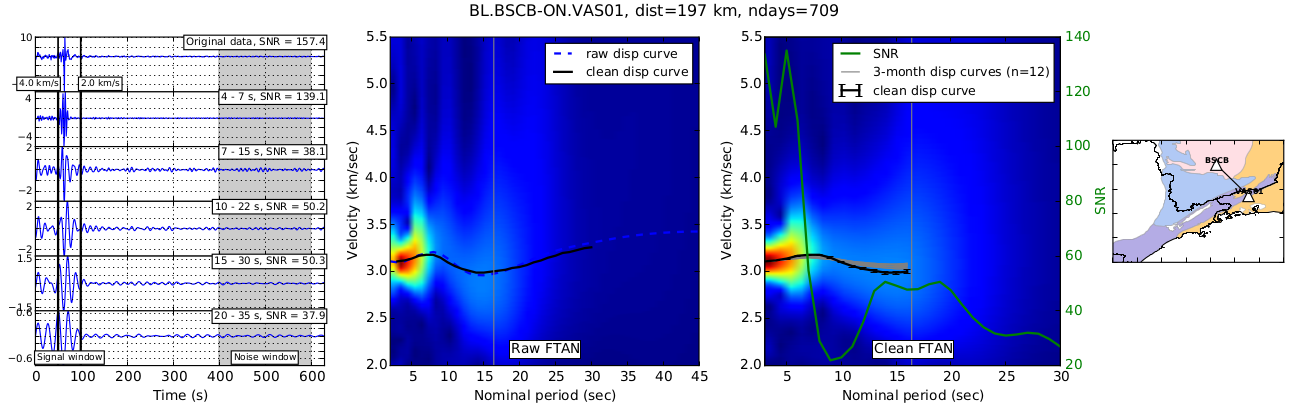
\includegraphics[scale=0.3]{Figs/correlacao_FTAN.png}
\caption[Exemplo de correlação cruzada e análise frequência-tempo (FTAN) no par de estações BL.BSCB-ON.PET01.]{Exemplo de correlação cruzada e análise frequência-tempo (FTAN) no par de estações BL.BSCB-ON.PET01. (Esquerda) Correlação cruzada original simetrizada e filtrada com passa-banda. (Centro) Amplitude da FTAN bruta e filtrada, normalizada por cada valor de período e curvas de dispersão das velocidades de grupo. Os dados da forma de onda foram filtradas entre 3 e 50 segundos.(Direita) Mapa mostrando a localização do par de estações (estações, províncias tectônicas e divisas estaduais).}
\label{correlacao_FTAN}
\end{figure}

A Figura \ref{correlacao_FTAN} ilustra todo o processo descrito acima no par de estações BL.BSCB-ON.PET01: cálculo das correlações cruzadas. FTAN bruta, FTAN filtrada, medidas das curvas de dispersão e avaliação da variabilidade sazonal. 

\subsection{Controle de Qualidade das Medidas}

Como a quantidade de caminhos entre as estações é numerosa, o controle de qualidade das correlações cruzadas deverá ser aplicado automaticamente, assim haverá o mínimo de interação humana, pois assim medidas errôneas serão minimizadas. \cite{bensen_processing_2007} mostra que medidas de dispersão confiáveis devem passar pelo seguinte critério: $\Delta > 3\lambda = 3c\tau$ ou $\tau < \Delta/3c$, sendo $\tau$ o período, $c$ o comprimento de onda, $\Delta$ a distância entre as estações em quilômetros e $\lambda$ o comprimento de onda. Sendo a velocidade de fase ($c$) $\sim 4 km/s$, o período máximo de trabalho é estabelecido por $\tau_{max} = \Delta/12$. \cite{bensen_processing_2007} observa uma degradação das medidas de dispersão em períodos maiores que $\tau_{max}$, como observado na Figura \ref{correlacao_FTAN}. 

Para o controle de qualidade dos dados, deve-se identificar e rejeitar medidas ruins. Junto com os critérios estabelecidos por \cite{bensen_processing_2007}, anteriormente, utilizou-se a razão sinal-ruído (SNR) . A definição de SNR é a razão entre o valor máximo absoluto na janela de sinal e o desvio padrão da janela de ruído. Estas janelas são estabelecidas de acordo com a distância entre as estações ($\Delta$). A janela de sinal é demarcada entre os tempos de chegada correspondentes as velocidades de 2.5 e 3.5 $km/s$, mostradas na Figura \ref{correlacao_cruzada}. A janela de ruído é demarcada 300 segundos após a janela de sinal, isso para garantir que seja apenas ruído. O SNR é calculado para cada período aplicando um filtro Gaussiano estreito centrado no período correspondente. As medidas da razão sinal-ruído são observadas na parte central da Figura \ref{correlacao_cruzada}. 

Outro critério estabelecido por \cite{bensen_processing_2007} é avaliar a repetibilidade temporal das medidas de dispersão. As fontes de ruído ambiental mudam sazonalmente e fornecem diferentes condições
para as medições. Dadas as condições de mudança, portanto, a repetibilidade da medição é um indicador significativo de confiabilidade. O procedimento utilizado foi a calcular o desvio padrão para um conjunto de velocidades sazonais que tenham SNR maior que 7 e que tenham no mínimo 3 dessas velocidades disponíveis. Se não for satisfeito esse critério o desvio padrão é considerado indefinido.

\subsection{Inversão Tomográfica}

A metodologia desenvolvida por  \cite{barmin_fast_2001} foi utilizada para produzir os mapas de velocidade de grupo das ondas Rayleigh. Assume-se que as ondas de superfície seguem os caminhos entre os pares de estações. Isto faz com que a inversão seja um problema linear em relação a vagarosidade. Então a relação entre um período $T$ qualquer é dada por:

\begin{equation}
d=Gm
\end{equation} 

O vetor $d$ contém o pertubações no tempo de viagem entre os pares de estações (deduzidos das velocidades de grupo medidas no período $T$), o vetor de parâmetro $m$ consite da pertubações na vagarosidade ao longo dos nós de um grade regular e a matriz sensibilidade $G$ realiza a integração entre a vagarosidade ao longo do caminho percorrido pelas ondas. As pertubações são relativas ao modelo de referência, definido como a vagarosidade média implícita por todos o tempos de propagação das ondas observados. A vagarosidade modelada é discretizada ao longo de uma grade regular de 1º x 1º. 

A função de penalização é composta por três termos:

\begin{eqnarray}
(Gm-d)^{T}C^{-1}(Gm-d) + \alpha ^{2} \left \| F(m)  \right \| ^{2} + \beta ^{2 } \left \| H(m)  \right \| ^{2}
\end{eqnarray}

O primeiro termo é o desajuste, $C$ é a matriz de covariância dos erros observacionais. $C$ é uma matriz diagonal contendo a variância dos erros nos tempos de viagens observados, que são deduzidos do desvio padrão das velocidade de grupo, estas calculadas previamente. 

O segundo termpo da função de penalização é a condição de suavidade espacial, que é dada por:

\begin{eqnarray}
F_{i}(m)=m_{i}-\sum_{j\neq i}S(r_{i},r_{j})m_{j}
\end{eqnarray}

com $r_{i}$ a posição do $i$-nt nós da grade e:

\begin{eqnarray}
S(r_{i},r_{j}) \propto exp(- \frac{\left \| r_{i}-r_{j}  \right \|^{2}}{2\sigma ^{2}}) \\
\sum_{j\neq i} S(r_{i},r_{j}) = 1         \forall i 
\end{eqnarray}


O terceiro termo penaliza a norma ponderada no modelo, isos faz com que o modelo suavize regiões onde há pouca cobertura de dados:

\begin{eqnarray}
H_{i}(m) = exp(-\lambda \rho _{i})m_{i}
\end{eqnarray}

onde $\rho _{i}$ é o número de caminhos que cruza a célula 1º x 1º centrada no $i$-nt nó da grade. Os parâmetros foram ajustados através de otimizações feitas por tentativa e erro.

Para identificar e remover caminhos discrepantes que podem ter passado pelo critério de seleção o procedimento passa-dois foi empregado. Inicialmente um mapa suave de velocidade é produzido através de uma inversão superamortecida. Nesta a maior parte da energia é afetada pela condição de suavidade espacial. Pares que possuem um tempo de viagem residual maior que três vezes o desvio padrão do resíduo, calculado pela diferença entre o tempo de viagem observado e predito,  são descartados. Após isso, uma segunda inversão é feita. O mapa de velocidade gerado por essa segunda inversão é o mapa de velocidade final. A porcentagem de medidas rejeitadas é menos que 2\% em todas as faixas de períodos.

\subsection{Análise da Resolução dos Mapas Tomográficos}

Antes de interpretar os resultados é necessário fazer uma análise da resolução dos dados. Com isso pode-se avaliar as limitações dos mapas tomográficos gerados. O processo de inversão descrito nas seções anteriores produz concomitantemente com o resultado uma matriz de resolução. Segundo \cite{barmin_fast_2001} ajusta-se um cone para cada mapa de resolução e reporta o raio deste cone como a resolução espacial característica, isto é interpretado como a distância de separação mínima para duas anomalias para ser resolvido. A resolução não pode ser menor que duas vezes o espaçamento entre os nós. Além disso, cones que possuem os melhores ajustes de altura menores que 10\% da altura máxima são considerados ruído e são automaticamente descartados.  

As limitações dos mapas tomográficos serão avaliadas qualitativamente pelo teste de tabuleiro de damas, \textit{checkerboard}, onde os tempos de viagem observados são substituídos por dados sintéticos gerados de um modelo de anomalias  de velocidade em forma de tabuleiro de damas. O modelo tem alternado anomalias senoidais de $\pm 10\% $em torno de um valor de velocidade padrão de 3 $kms^{-1}$. Em geral, as limitações descritas pelos tabuleiros reconstruídos são consistentes com a resolução espacial estimada.